\section{Architecture}

Socneto is a distributed application, the whole platform is robust and components are loosely coupled. Application is divided into services by their functionality. Everything is connected via Kafka messaging \ref{subsection:messaging} or internal REST API.

\subsection{Components}

Socneto is divided into eight logical parts:

\begin{itemize}
    \item Messaging (see Subsection \ref{subsection:messaging})
    \item Frontend (see Section \ref{section:frontend})
    \item Backend (see Section \ref{section:backend})
    \item Job managing service (see Section \ref{section:jms})
    \item Multiple data acquiring components (see Section \ref{section:acquirers})
    \item Multiple data analysers (see Section \ref{section:analysers}) 
    \item Storage (see Section \ref{section:storage})
    \item Monitoring (see Section \ref{section:monitoring})
\end{itemize}

Socneto can be extended by adding custom data acquirers or data analysers (for more details, see Section \ref{section:extensibility}). 

\subsection{Component Relationships}

The communication among the components respects the data flow of the application. A user submits a job through frontend to backend which notifies job management service (JMS). JMS then notifies all selected data acquirers and data analysers. The data analysers start to produce posts that start to flow into data analysers and to the storage. The analysers consume posts and produce analyses that are also sent to the storage. The storage consumes the posts and analyses and offers them to the user's queries through backend query endpoints. These relationships can be seen in Figure \ref{fig:concept}.

\begin{figure}[ht]
    \centering
    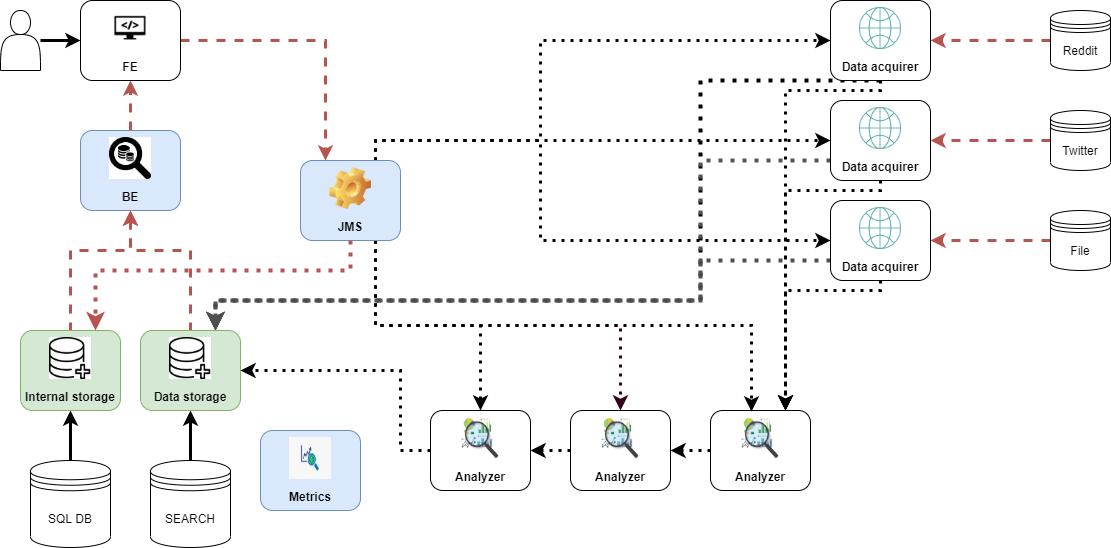
\includegraphics[width=\textwidth]{diagrams/soc-all.png}
        \caption{A diagram of the Socneto architecture showing relation ships among all components. This communication is asynchronous}
        \label{fig:concept}
\end{figure}

\subsection{Messaging}\label{subsection:messaging}

\paragraph{Publish \& Subscribe Principle}

\textit{"Publish/subscribe messaging, or pub/sub messaging, is a form of asynchronous service-to-service communication used in serverless and microservices architectures. In a pub/sub model, any message published to a topic is immediately received by all of the subscribers to the topic. Pub/sub messaging can be used to enable event-driven architectures, or to decouple applications in order to increase performance, reliability and scalability."}\footnote{\url{https://aws.amazon.com/pub-sub-messaging/}}

\paragraph{Publish/Subscribe in our Use-Case}

Posts are acquired and asynchronously sent to analysers and storage. Analysers subscribe to their assigned queues and after each analysis, they also send results to storage via messaging. Using this approach we achieved better extensibility of Socneto, high-throughput and loose coupling between modules. Defined message structures are described in Appendix \ref{appendix}. Acquirers and analysers get assigned topics during a registration and update processes.

\paragraph{Implementation}

In Socneto we have chosen Apache Kafka 2.4.0\footnote{\url{https://kafka.apache.org}} for messaging, which is an open-source project from Hadoop family\footnote{\url{https://hadoop.apache.org}} developed by Linkedin and the platform meets our requirements. Also, all common languages have a library with a connector to  Kafka.

\section{Project Structure}\label{section:projectStructure}

The project has the following directories
\begin{itemize}
    \item \texttt{acquisition} - Data acquirer code
    \item \texttt{analysers} - Data analyser code
    \item \texttt{backend} - Backend code
    \item \texttt{docs} - Documentation
    \item \texttt{frontend} - Frontend code
    \item \texttt{job-management} - Job Management Service code
    \item \texttt{storage} - Storage related code
    \item \texttt{tests} - Tests
\end{itemize}